% ĐỀ KIỂM TRA GIỮA KÌ 1 MÔN TOÁN 12 - MÃ ĐỀ 101 (CHUẨN BỘ GIÁO DỤC VÀ ĐÀO TẠO)
% PHẦN I: TRẮC NGHIỆM NHIỀU PHƯƠNG ÁN LỰA CHỌN (12 CÂU)

\begin{ex}
    Cho hàm số $y = f(x)$ có bảng biến thiên như sau:
    \begin{center}
    
\begin{tikzpicture}
        \tkzTabInit[lgt=1.5,espcl=2.2]{$x$/0.8,$y'$/0.8,$y$/1.5}{$-\infty$,$-1$,$1$,$+\infty$}
        \tkzTabLine{,+,$0$,-,$0$,+,}
        \tkzTabVar{-/$-\infty$,+/3,-/$-1$,+/$+\infty$}
    \end{tikzpicture}
    \end{center}
    Hàm số đã cho đồng biến trên khoảng nào dưới đây?
    \choice
    {$(-1; 1)$}
    {\True $(1; +\infty)$}
    {$(-\infty; 1)$}
    {$(-1; +\infty)$}
    \loigiai{Dựa vào bảng biến thiên, hàm số đồng biến trên các khoảng $(-\infty; -1)$ và $(1; +\infty)$. Do đó chọn $(1; +\infty)$.}
\end{ex}

\begin{ex}
    Cho hàm số bậc ba $y = f(x) = x^3 - 3x$ có đồ thị như hình vẽ bên dưới:
    \begin{center}
    \begin{tikzpicture}
        \draw[->] (-3,0) -- (3,0) node[below] {$x$};
        \draw[->] (0,-3) -- (0,3) node[right] {$y$};
        \draw (0,0) node[below left] {$O$};
        \draw[dashed] (-1,0) -- (-1,2) -- (0,2);
        \draw[dashed] (1,0) -- (1,-2) -- (0,-2);
        \draw[smooth,domain=-2.1:2.1,blue,thick] plot(\x, {(\x)^3 - 3*(\x)});
    \end{tikzpicture}
    \end{center}
    Điểm cực đại của đồ thị hàm số đã cho là:
    \choice
    {\True $(-1; 2)$}
    {$(1; -2)$}
    {$x = -1$}
    {$y = 2$}
    \loigiai{Từ đồ thị, điểm cực đại của đồ thị hàm số là $(-1; 2)$.}
\end{ex}

\begin{ex}
    Giá trị lớn nhất của hàm số $f(x) = x^4 - 2x^2 + 3$ trên đoạn $[0; 2]$ bằng:
    \choice
    {$3$}
    {$2$}
    {\True $11$}
    {$12$}
    \loigiai{Ta có $f'(x) = 4x^3 - 4x = 0 \Leftrightarrow x = 0$ hoặc $x = 1$ trên $[0; 2]$. Ta có $f(0) = 3$, $f(1) = 2$, $f(2) = 11$. Vậy giá trị lớn nhất bằng $11$.}
\end{ex}

\begin{ex}
    Đường tiệm cận ngang của đồ thị hàm số $y = \dfrac{3x - 1}{x + 2}$ có phương trình là:
    \choice
    {$x = -2$}
    {\True $y = 3$}
    {$y = -2$}
    {$x = 3$}
    \loigiai{Ta có $\lim_{x \to \pm\infty} \dfrac{3x - 1}{x + 2} = 3$, do đó đường tiệm cận ngang là $y = 3$.}
\end{ex}

\begin{ex}
    Cho hàm số $y = f(x)$ liên tục trên đoạn $[-2; 3]$ và có đồ thị như hình vẽ:
    \begin{center}
    \begin{tikzpicture}
        \draw[->] (-3,0) -- (4,0) node[below] {$x$};
        \draw[->] (0,-3) -- (0,5) node[right] {$y$};
        \draw (0,0) node[below left] {$O$};
        \draw[dotted] (-2,0) -- (-2,1) -- (0,1);
        \draw[dotted] (-1,0) -- (-1,3) -- (0,3);
        \draw[dotted] (1,0) -- (1,-2) -- (0,-2);
        \draw[dotted] (3,0) -- (3,4) -- (0,4);
        \draw[thick,red] (-2,1) to[out=60,in=180] (-1,3) to[out=0,in=180] (1,-2) to[out=0,in=240] (3,4);
    \end{tikzpicture}
    \end{center}
    Gọi $M$ và $m$ lần lượt là giá trị lớn nhất và giá trị nhỏ nhất của hàm số trên đoạn $[-2; 3]$. Giá trị của $M + m$ bằng:
    \choice
    {$1$}
    {\True $2$}
    {$5$}
    {$7$}
    \loigiai{Dựa vào đồ thị hàm số trên đoạn $[-2; 3]$, ta thấy giá trị lớn nhất $M = 4$ tại $x = 3$, và giá trị nhỏ nhất $m = -2$ tại $x = 1$. Suy ra $M + m = 4 + (-2) = 2$.}
\end{ex}

\begin{ex}
    Cho hàm số $y = f(x)$ có bảng biến thiên:
    \begin{center}
    
\begin{tikzpicture}
        \tkzTabInit[lgt=1.5,espcl=2]{$x$/0.8,$y'$/0.8,$y$/1.5}{$-\infty$,$1$,$+\infty$}
        \tkzTabLine{,-,d,-,}
        \tkzTabVar{+/2,-D/ $-\infty$ / $+\infty$,-/2}
    \end{tikzpicture}
    \end{center}
    Tổng số đường tiệm cận đứng và tiệm cận ngang của đồ thị hàm số là:
    \choice
    {$1$}
    {\True $2$}
    {$3$}
    {$4$}
    \loigiai{Đồ thị hàm số có 1 đường tiệm cận đứng $x = 1$ và 1 đường tiệm cận ngang $y = 2$. Tổng số đường tiệm cận là $2$.}
\end{ex}

\begin{ex}
    Tìm tất cả các giá trị của tham số $m$ để hàm số $y = \dfrac{x + 2m}{x - 1}$ đồng biến trên từng khoảng xác định.
    \choice
    {$m > -\dfrac{1}{2}$}
    {\True $m < -\dfrac{1}{2}$}
    {$m \ge -\dfrac{1}{2}$}
    {$m \le -\dfrac{1}{2}$}
    \loigiai{Tập xác định $D = \mathbb{R} \setminus \{1\}$. Đạo hàm $y' = \dfrac{-1 - 2m}{(x - 1)^2}$. Hàm số đồng biến khi $-1 - 2m > 0 \Leftrightarrow m < -\dfrac{1}{2}$.}
\end{ex}

\begin{ex}
    Cho khối lập phương có cạnh bằng $a$. Thể tích của khối lập phương đã cho bằng:
    \choice
    {$\dfrac{1}{3}a^3$}
    {$a^2$}
    {\True $a^3$}
    {$3a^3$}
    \loigiai{Thể tích khối lập phương có cạnh $a$ là $V = a^3$.}
\end{ex}

\begin{ex}
    Cho khối chóp $S.ABC$ có đáy $ABC$ là tam giác vuông tại $B$, $AB = a$, $BC = 2a$. Chiều cao $SA = 3a$. Thể tích khối chóp đã cho bằng:
    \choice
    {$3a^3$}
    {$2a^3$}
    {\True $a^3$}
    {$\dfrac{1}{3}a^3$}
    \loigiai{Diện tích đáy $S_{\triangle ABC} = \dfrac{1}{2} \cdot a \cdot 2a = a^2$. Thể tích $V = \dfrac{1}{3} S \cdot h = \dfrac{1}{3} \cdot a^2 \cdot 3a = a^3$.}
\end{ex}

\begin{ex}
    Cho hàm số phân thức bậc nhất trên bậc nhất $y = \dfrac{2x - 1}{x + 1}$ có đồ thị như hình vẽ:
    \begin{center}
    \begin{tikzpicture}
        \draw[->] (-5,0) -- (5,0) node[below] {$x$};
        \draw[->] (0,-4) -- (0,5) node[right] {$y$};
        \draw (0,0) node[below left] {$O$};
        \draw[dashed,red] (-1,-4) -- (-1,5);
        \draw[dashed,red] (-5,2) -- (5,2);
        \draw[smooth,domain=-4.5:-1.2,blue,thick] plot(\x, {(2*\x-1)/(\x+1)});
        \draw[smooth,domain=-0.8:4.5,blue,thick] plot(\x, {(2*\x-1)/(\x+1)});
    \end{tikzpicture}
    \end{center}
    Tọa độ giao điểm của hai đường tiệm cận của đồ thị hàm số là:
    \choice
    {$(1; 2)$}
    {\True $(-1; 2)$}
    {$(2; -1)$}
    {$(-1; -1)$}
    \loigiai{Tiệm cận đứng là $x = -1$, tiệm cận ngang là $y = 2$. Do đó giao điểm của hai đường tiệm cận là $(-1; 2)$.}
\end{ex}

\begin{ex}
    Cho khối chóp tứ giác đều có cạnh đáy bằng $a$ và cạnh bên bằng $a\sqrt{2}$. Chiều cao của khối chóp bằng:
    \choice
    {$\dfrac{a}{2}$}
    {\True $\dfrac{a\sqrt{6}}{2}$}
    {$a\sqrt{2}$}
    {$\dfrac{a\sqrt{3}}{2}$}
    \loigiai{Bán kính đường tròn ngoại tiếp đáy $R = \dfrac{a\sqrt{2}}{2}$. Chiều cao $h = \sqrt{b^2 - R^2} = \sqrt{2a^2 - \dfrac{a^2}{2}} = \dfrac{a\sqrt{6}}{2}$.}
\end{ex}

\begin{ex}
    Đồ thị hàm số nào sau đây có dạng đường cong hình chữ $W$?
    \choice
    {$y = x^3 - 3x + 1$}
    {$y = -x^4 + 2x^2 + 1$}
    {\True $y = x^4 - 2x^2 - 1$}
    {$y = \dfrac{x + 1}{x - 1}$}
    \loigiai{Hàm số trùng phương $y = ax^4 + bx^2 + c$ với $a > 0$ và $ab < 0$ có 3 điểm cực trị và đồ thị dạng chữ $W$. Do đó hàm số $y = x^4 - 2x^2 - 1$ thỏa mãn.}
\end{ex}

% PHẦN II: CÂU TRẮC NGHIỆM ĐÚNG SAI (4 CÂU)

\begin{ex}
    Cho hàm số bậc ba $y = f(x) = ax^3 + bx^2 + cx + d$ ($a \ne 0$) có đồ thị như hình vẽ bên:
    \begin{center}
    \begin{tikzpicture}
        \draw[->] (-3,0) -- (3,0) node[below] {$x$};
        \draw[->] (0,-3) -- (0,4) node[right] {$y$};
        \draw (0,0) node[below left] {$O$};
        \draw (0,1) node[left] {$d$};
        \draw[smooth,domain=-2.2:2.3,blue,thick] plot(\x, {0.6*(\x)^3 - 1.8*(\x) + 1});
    \end{tikzpicture}
    \end{center}
    Xét tính đúng hay sai của các mệnh đề sau:
    \choiceTFt
    {\True Hệ số $a > 0$.}
    {\True Đồ thị cắt trục tung tại điểm có tung độ $d > 0$.}
    {Hàm số có hai điểm cực trị cùng dấu.}
    {\True Phương trình $f(x) = 0$ có 3 nghiệm phân biệt.}
    \loigiai{
        Nhánh cuối của đồ thị đi lên nên $a > 0$ (Đúng).\\
        Đồ thị cắt $Oy$ tại $(0; d)$ phía trên trục hoành nên $d > 0$ (Đúng).\\
        Hai điểm cực trị nằm về hai phía của trục tung nên trái dấu (Mệnh đề nói cùng dấu là Sai).\\
        Đồ thị cắt trục hoành tại 3 điểm phân biệt nên phương trình $f(x) = 0$ có 3 nghiệm phân biệt (Đúng).
    }
\end{ex}

\begin{ex}
    Cho hàm số $y = f(x)$ có đạo hàm $f'(x) = x(x - 1)^2 (x + 2)^3$.
    Xét tính đúng hay sai của các mệnh đề sau:
    \choiceTFt
    {\True Phương trình $f'(x) = 0$ có 3 nghiệm thực.}
    {\True Hàm số đã cho có đúng 2 điểm cực trị.}
    {Hàm số đạt cực đại tại điểm $x = 0$.}
    {\True Hàm số đồng biến trên khoảng $(0; +\infty)$.}
    \loigiai{
        Nghiệm của $f'(x) = 0$ là $x = 0$, $x = 1$, $x = -2$ (Đúng).\\
        Nghiệm bội chẵn $x = 1$ không làm đổi dấu đạo hàm; $x = 0$ và $x = -2$ là nghiệm bội lẻ nên là điểm cực trị $\Rightarrow$ có 2 điểm cực trị (Đúng).\\
        Qua $x = 0$, $f'(x)$ đổi dấu từ âm sang dương nên $x = 0$ là điểm cực tiểu (Mệnh đề cực đại là Sai).\\
        Với $x > 0$, $x > 0$, $(x-1)^2 \ge 0$, $(x+2)^3 > 0 \Rightarrow f'(x) \ge 0 \Rightarrow$ hàm số đồng biến trên $(0; +\infty)$ (Đúng).
    }
\end{ex}

\begin{ex}
    Bảng thống kê sau đây cho biết thời gian hoàn thành một bài kiểm tra Toán của 40 học sinh lớp 12:
    \begin{center}
    \begin{tabular}{|c|c|c|c|c|}
    \hline
    Thời gian (phút) & $[20; 25)$ & $[25; 30)$ & $[30; 35)$ & $[35; 40)$ \\
    \hline
    Số học sinh & $6$ & $14$ & $12$ & $8$ \\
    \hline
    \end{tabular}
    \end{center}
    Xét tính đúng hay sai của các mệnh đề sau:
    \choiceTFt
    {\True Nhóm chứa mốt của mẫu số liệu ghép nhóm là $[25; 30)$.}
    {\True Cỡ mẫu của số liệu trên là $n = 40$.}
    {Giá trị đại diện của nhóm $[30; 35)$ bằng $32$.}
    {\True Đa số học sinh hoàn thành bài kiểm tra trong khoảng từ 25 đến 35 phút.}
    \loigiai{
        Tần số lớn nhất là 14 ứng với nhóm $[25; 30)$ nên nhóm chứa mốt là $[25; 30)$ (Đúng).\\
        Tổng tần số $6 + 14 + 12 + 8 = 40$ (Đúng).\\
        Giá trị đại diện của nhóm $[30; 35)$ là $\dfrac{30 + 35}{2} = 32.5$ (Mệnh đề bằng 32 là Sai).\\
        Số học sinh trong khoảng từ 25 đến 35 phút là $14 + 12 = 26/40 = 65\%$ (Đa số - Đúng).
    }
\end{ex}

\begin{ex}
    Cho hàm số $y = \dfrac{x^2 + 2x + 2}{x + 1}$.
    Xét tính đúng hay sai của các mệnh đề sau:
    \choiceTFt
    {\True Đồ thị hàm số có tiệm cận xiên là đường thẳng $y = x + 1$.}
    {\True Đồ thị hàm số có tiệm cận đứng là đường thẳng $x = -1$.}
    {Hàm số nghịch biến trên khoảng $(0; +\infty)$.}
    {\True Tâm đối xứng của đồ thị là điểm $I(-1; 0)$.}
    \loigiai{
        Biến đổi $y = x + 1 + \dfrac{1}{x + 1}$. Tiệm cận xiên $y = x + 1$ (Đúng).\\
        Tiệm cận đứng $x = -1$ (Đúng).\\
        Đạo hàm $y' = 1 - \dfrac{1}{(x + 1)^2} = \dfrac{x(x + 2)}{(x + 1)^2} > 0$ trên $(0; +\infty)$ nên hàm số đồng biến (Mệnh đề nghịch biến là Sai).\\
        Tọa độ giao điểm hai tiệm cận là nghiệm của hệ $\begin{cases} x = -1 \\ y = x + 1 \end{cases} \Rightarrow I(-1; 0)$ là tâm đối xứng (Đúng).
    }
\end{ex}

% PHẦN III: CÂU TRẮC NGHIỆM TRẢ LỜI NGẮN (4 CÂU)

\begin{ex}
    Cho hàm số $y = f(x) = x^3 - 3x^2 + 2$. Điểm cực tiểu của đồ thị hàm số có tung độ bằng bao nhiêu?
    \begin{center}
    \begin{tikzpicture}
        \draw[->] (-2,0) -- (4,0) node[below] {$x$};
        \draw[->] (0,-4) -- (0,4) node[right] {$y$};
        \draw (0,0) node[below left] {$O$};
        \draw[dashed] (2,0) -- (2,-2) -- (0,-2);
        \draw[smooth,domain=-1:3.2,blue,thick] plot(\x, {(\x)^3 - 3*(\x)^2 + 2});
    \end{tikzpicture}
    \end{center}
    \shortans{-2}
    \loigiai{Ta có $y' = 3x^2 - 6x = 0 \Leftrightarrow x = 0$ hoặc $x = 2$. Với $x = 2$ thì $y(2) = 2^3 - 3(2^2) + 2 = -2$. Tung độ điểm cực tiểu là $-2$.}
\end{ex}

\begin{ex}
    Tìm nghiệm của phương trình $\log_3(2x - 1) = 2$.
    \shortans{5}
    \loigiai{Điều kiện $x > \dfrac{1}{2}$. Phương trình tương đương $2x - 1 = 3^2 = 9 \Leftrightarrow 2x = 10 \Leftrightarrow x = 5$.}
\end{ex}

\begin{ex}
    Cho hàm số $y = x^3 - 3x^2 + 3$ có đồ thị $(C)$. Tìm giá trị cực tiểu của hàm số đã cho.
    \begin{center}
    \begin{tikzpicture}
        \draw[->] (-2,0) -- (4,0) node[below] {$x$};
        \draw[->] (0,-2) -- (0,5) node[right] {$y$};
        \draw (0,0) node[below left] {$O$};
        \draw[dashed] (2,0) -- (2,-1) -- (0,-1);
        \draw[smooth,domain=-1:3.2,blue,thick] plot(\x, {(\x)^3 - 3*(\x)^2 + 3});
    \end{tikzpicture}
    \end{center}
    \shortans{-1}
    \loigiai{Ta có $y' = 3x^2 - 6x = 0 \Leftrightarrow x = 0$ hoặc $x = 2$. Giá trị cực tiểu đạt tại $x = 2$, suy ra $y_{CT} = y(2) = 8 - 12 + 3 = -1$.}
\end{ex}

\begin{ex}
    Một hình nón có bán kính đáy $r = 3$ cm và chiều cao $h = 4$ cm. Tính diện tích xung quanh của hình nón theo đơn vị $\pi\text{ cm}^2$.
    \shortans{15}
    \loigiai{Đường sinh $l = \sqrt{r^2 + h^2} = \sqrt{3^2 + 4^2} = 5$ cm. Diện tích xung quanh $S_{xq} = \pi r l = \pi \cdot 3 \cdot 5 = 15\pi\text{ cm}^2$. Kết quả cần điền là $15$.}
\end{ex}

% PHẦN IV: CÂU HỎI ĐIỀN KHUYẾT VÀ TỰ LUẬN (3 CÂU)

\begin{ex}
    Đường thẳng $x = x_0$ được gọi là đường tiệm cận [...] của đồ thị hàm số $y = f(x)$ nếu ít nhất một trong các điều kiện sau được thỏa mãn: $\lim_{x \to x_0^+} f(x) = +\infty$, $\lim_{x \to x_0^+} f(x) = -\infty$, $\lim_{x \to x_0^-} f(x) = +\infty$, hoặc $\lim_{x \to x_0^-} f(x) = -\infty$.
    \cloze{đứng}
    \loigiai{Theo định nghĩa hình học giải tích Toán 12, đường thẳng $x = x_0$ là đường tiệm cận đứng.}
\end{ex}

\begin{ex}
    Khảo sát sự biến thiên và vẽ đồ thị của hàm số $y = x^3 - 3x^2 + 2$.
    \loigiai{
        1. Tập xác định: $D = \mathbb{R}$.\\
        2. Sự biến thiên:\\
        - Chiều biến thiên: $y' = 3x^2 - 6x = 3x(x - 2)$. Cho $y' = 0 \Leftrightarrow x = 0$ hoặc $x = 2$.\\
        - Khoảng đồng biến: $(-\infty; 0)$ và $(2; +\infty)$; Khoảng nghịch biến: $(0; 2)$.\\
        - Cực trị: Hàm số đạt cực đại tại $x = 0, y_{CĐ} = 2$; đạt cực tiểu tại $x = 2, y_{CT} = -2$.\\
        - Giới hạn: $\lim_{x \to -\infty} y = -\infty; \lim_{x \to +\infty} y = +\infty$.\\
        3. Điểm uốn và đồ thị: $y'' = 6x - 6 = 0 \Leftrightarrow x = 1 \Rightarrow I(1; 0)$ là tâm đối xứng.
    }
\end{ex}

\begin{ex}
    Một xí nghiệp muốn thiết kế một thùng chứa hình trụ bằng kim loại có thể tích $V = 16\pi\text{ dm}^3$. Hãy xác định bán kính đáy $R$ (theo dm) sao cho diện tích toàn phần của thùng chứa đạt giá trị nhỏ nhất (để tiết kiệm nguyên vật liệu nhất).
    \begin{center}
    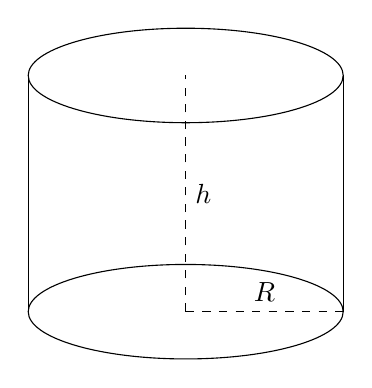
\begin{tikzpicture}
        \draw (0,0) ellipse (2cm and 0.6cm);
        \draw (0,3) ellipse (2cm and 0.6cm);
        \draw (-2,0) -- (-2,3);
        \draw (2,0) -- (2,3);
        \draw[dashed] (0,0) -- (2,0) node[midway,above] {$R$};
        \draw[dashed] (0,0) -- (0,3) node[midway,right] {$h$};
    \end{tikzpicture}
    \end{center}
    \loigiai{
        Thể tích khối trụ: $V = \pi R^2 h = 16\pi \Rightarrow h = \dfrac{16}{R^2}$.\\
        Diện tích toàn phần: $S_{tp} = 2\pi R^2 + 2\pi R h = 2\pi R^2 + 2\pi R \left(\dfrac{16}{R^2}\right) = 2\pi \left(R^2 + \dfrac{16}{R}\right) = 2\pi \left(R^2 + \dfrac{8}{R} + \dfrac{8}{R}\right)$.\\
        Áp dụng bất đẳng thức AM-GM (Cauchy) cho 3 số dương:\\
        $R^2 + \dfrac{8}{R} + \dfrac{8}{R} \ge 3 \sqrt[3]{R^2 \cdot \dfrac{8}{R} \cdot \dfrac{8}{R}} = 3 \sqrt[3]{64} = 3 \cdot 4 = 12$.\\
        Đẳng thức xảy ra khi và chỉ khi $R^2 = \dfrac{8}{R} \Leftrightarrow R^3 = 8 \Leftrightarrow R = 2\text{ (dm)}$.\\
        Khi đó $h = \dfrac{16}{2^2} = 4\text{ (dm)}$. Vậy $R = 2\text{ dm}$.
    }
\end{ex}
